
\documentclass{mise_en_page}
\usepackage[utf8]{inputenc}
\usepackage[T1]{fontenc}
\usepackage[french]{babel}
\usepackage{amsmath}
\usepackage{amssymb,amsfonts,textcomp}
\usepackage{array}
\usepackage{hhline}

\projet{Projet Ingéniérie}
\equipe{H4314}
\responsable{Tristan Delizy}
\titre{Dossier d'initialisation}
\version{1.1}
\objet{mise en place des phases et activités du projet.}
\etat{validé} %draft, non relu, non validé, validé

\begin{document}

\maketitle

\begin{historique}
    \histo{1.0}{16/01/2012}{Draft initial}
    \histo{1.1}{23/01/2012}{Finalisation}
    \histo{1.2}{30/01/2012}{Validation}
\end{historique}

\newpage

\tableofcontents

\section{Contexte}
\ \ L’Union Européenne possède de vastes territoires et certains sites
sont isolés difficiles d’accès et possèdent un climat extrême. Le
Comité pour la Protection de l’EnVironnement de l’UE (COPEVUE) à émis
un appel d’offre pour l’étude d’un système de monitoring à distance des
sites isolés. Dans ces zones peu peuplées, isolées et difficiles
d’accès, l’union européenne souhaite pouvoir intervenir et récupérer
des informations rapidement, efficacement et durablement.

\ \ La proposition à laquelle aboutira notre étude devra faciliter
l’autonomie de tels sites et leur permettre un fonctionnement plus aisé
et plus optimal. Le système étudié doit être fiable et robuste, en
effet, certaines fonctions qu’il assurera aura des conséquences directe
sur des secteurs aussi importants que la lutte contre les incendies.

\ \ Un point important du contexte dans lequel le projet doit se situer
est l’aspect européen du projet. Le système à déployer doit s’adapter
aux différents réseaux présents en Europe, doit proposer à minima une
interface compréhensible par tous (en anglais)  et correspondre aux
normes européennes. En effet nous ne connaissons pas à priori
l’emplacement de chaque site où sera utilisé le système, celui-ci devra
donc dans l’idéal pouvoir s’adapter aux différentes normes réseaux
mises en places au sein de l’union européenne. de plus, certains
matériels devront utiliser les infrastructures spécifiques à un site et
donc pouvoir s’y adapter (modularité des capteurs, installation aisée).

\ \ Ainsi ce projet devra être hautement adaptable aux situations et aux
conditions environnementales tout en restant efficace, stable et
robuste, proposant une solution innovante apte à répondre aux besoins
du COPEVUE dans des délais relativement courts en maîtrisant les coûts
de l’étude et ceux de la réalisation.

\section{Objectif du projet}
Le travail réalisé durant ce projet par l’ensemble du groupe d’étude que
nous constituons est de réaliser un système permettant le monitoring de
sites isolés dans l’union européenne. le COPEVUE fournit dans son appel
d’offre quelques exemples de sites d’implantation du système. ceux-ci
sont des lieux où les conditions climatiques sont très contraignantes,
et la variété de ces conditions influerons fortement sur le matériel et
le système mis à l’étude.

Ce projet vise à étudier et concevoir un système complet autonome et
générique de mesure et de monitoring à distance de stations ainsi que
le pilotage, la configuration et la maintenance à distance de ces
stations. L’accent est mis sur l’évolutivité de la solution, son
autonomie et sa fiabilité.

Notre objectif ici est de répondre à l’appel d’offre émis par le Comité
pour la protection de l’EnVironnement de l’UE (COPEVUE) sous
l’identification “COPEVUE.2011.11.03.B”, rédigé par Mr Marian Scuturici
et approuvé par Mr Regis Aubry.

\subsection{rappel des exigences}
Le système proposé pour répondre à l’appel d’offre devra fournir les
fonctions suivantes : 

\begin{itemize}
\item Monitoring à distance
\item Maintenance à distance
\item Maintenance sur site
\item Traitements sur site central
\item Traitements sur station
\item Traçabilité
\item Logistique / optimisation des opérations
\item Aide à la décision.
\end{itemize}
\section{Phasage du projet}
\ \ Les phases proposées ici correspondent à la première partie du
projet, jusqu’à la revue intermédiaire. Elles concernent l’équipe aux
complet et se décomposent en tâches à effectuer, décrite dans la
section V (Tâches et activités) de ce document.

\subsection[PHASE 1 : INITIALISATION]{PHASE 1 : INITIALISATION}
\ \ Phase préliminaire du projet, basée sur la présentation en
amphithéatre et l’assistance par rôle en semaines 49 et 50. L’objectif
de cette phase est de préparer le travail de tous, de donner un cadre à
la rédaction des différents dossiers et d{\textquotesingle}appréhender
les moyens techniques existants déjà mis en oeuvre.

\subsection[PHASE 2 : ETUDE DE FAISABILITE]{PHASE 2 : ETUDE DE
FAISABILITE}
\ \ Cette deuxième phase est à but explorative pour le groupe d’étude
informatique qui doit soulever les différents problèmes à résoudre pour
répondre à l’appel d’offre. Durant cette phase le responsable qualité
et le chef de projet continuent le travail de balisage du projet et
mettent en place des outils de gestion de projet ou de suivi qualité.

\subsection[PHASE 3 : SPECIFICATION TECHNIQUE DES BESOINS]{PHASE 3 :
SPECIFICATION TECHNIQUE DES BESOINS}
\ \ La troisième phase correspond à la rédaction de livrables pour le
chef de projet, le groupe d’étude informatique doit quand à lui
apporter des solutions aux problèmes soulevés durant l’étude de
faisabilité. Le responsable qualité doit engager la réflection et
l’élaboration du plan d’assurance qualité logicielle. Cette phase
permet de cerner, non plus le projet ou le domaine d’application, mais
bien la solution apportée à l’appel d’offre.

\subsection[PHASE 4 : SYNTHESE DE LA SOLUTION]{PHASE 4 : SYNTHESE DE
LA SOLUTION}
\ \ Dernière phase de la première partie du projet (avant la revue
intermédiaire) la phase de synthèse de la solution correspond à la
finalisation des différents documents et à l’approfondissement de
l’étude de la solution répondant à l’appel d’offre.

\section[Livrables première partie]{Livrables première partie}
Cette section regroupe une description rapide des différents livrables
de la première partie du projet ingénierie 4IF, concernant la réponse à
l’appel d’offre émis par COPEVUE. Sont présentés ici les principaux
documents avec leur sommaire le cas échéant.

\subsection[Dossier de gestion de la documentation]{Dossier de
gestion de la documentation}
\paragraph[description générale]{description générale}
Ce dossier a pour but d’organiser la gestion ainsi que la production de
la documentation au sein du projet.

\paragraph[sommaire]{sommaire}
\begin{enumerate}
\item objectifs du dossier
\item acteurs de la gestion de documentation
\item cycle de vie d’un document
\item identification et structure d’un document
\item gestion des révisions
\item production de documents
\end{enumerate}
\subsection[Relevé de décisions]{Relevé de décisions}
\paragraph[description générale]{description générale}
\ \ Document bilan permettant de retracer et justifier les choix
(technologiques, architecturaux, etc...) de l’équipe au cours du
projet. document à vocation interne.

\paragraph[sommaire]{sommaire}
\begin{enumerate}
\item Objet
\item Séance 1
\item Séance 2
\item Séance 3
\end{enumerate}
\subsection[Fiche d’argumentation commerciale]{Fiche d’argumentation
commerciale}
\paragraph[description générale]{description générale}
\ \ La fiche d’argumentation commerciale est un livrable présentant de
manière courte le produit que nous proposons en réponse à l’appel
d’offre, mettant en avant les points forts de notre solution. Elle n’a
en aucun cas pour but de résumer les dossiers techniques qu’elle
accompagne, mais elle s’axe surtout autour de l’aspect commercial du
produit.

\subsection[Procédure d’aide à la décomposition d’un système en
sous{}-systèmes]{Procédure d’aide à la décomposition d’un système en
sous-systèmes}
\paragraph[description générale]{description générale}
\ \ Ce document à pour but de synthétiser la procédure à suivre en tant
que chef de projet pour décomposer un projet d’une taille conséquente
en sous-systèmes plus facilement analysable et dont les solutions sont
plus facilement accessibles. La rédaction de cette procédure appartient
donc à la gestion de la connaissance attenante à un projet et à pour
but de faciliter le rôle de chef de projet dans de futurs projets. Ce
document se base sur la best-practice rédigée par le responsable
qualité “aide à la rédaction d’une procédure”.

\paragraph[sommaire]{sommaire}
\begin{enumerate}
\item Objet
\item Documents de référence
\item Domaine d’application
\item Logigramme de la procédure
\item Tableau de définition des actions
\end{enumerate}
\subsection[Best{}-practice : Aide à la réalisation d’une
procédure]{Best-practice : Aide à la réalisation d’une procédure}
\paragraph[description générale]{description générale}
\ \ Définir les règles de rédaction d’une procédure devant intégrer le
système documentaire dans le cadre du projet COPEVUE-MONIT. Ce document
sera utilisé par le chef de projet dans le cadre de la rédaction de la
procédure d’aide à la décomposition d’un système en sous-systèmes.

\paragraph[sommaire]{sommaire}
\begin{enumerate}
\item définitions
\item documents de référence
\item méthode de rédaction
\item contenu d’une procédure
\item gestion du document
\end{enumerate}
\subsection[Dossier n°1]{Dossier n°1}
\paragraph[description générale]{description générale}
\ \ Premier dossier de retour de l’appel d’offre, ce dossier décrit la
première approche du projet, détaillant les solutions existantes, il
permet de réaliser une synthèse de la faisabilité du projet et de
mettre en avant des axes à privilégier dans la recherche de solutions

\paragraph[sommaire]{sommaire}
\begin{enumerate}
\item Etude de l’existant
\item Etude de faisabilité
\item Axes d’amélioration et thèmes de progrès
\end{enumerate}
\subsection[Dossier n°2]{Dossier n°2}
\paragraph[description générale]{description générale}
\ \ Le dossier n°2 correspond à une première réflexion sur la solution à
apporter à l’appel d’offre. Repartant des axes d’améliorations dégagés
dans le dossier n°1, il permet de spécifier les besoins techniques de
notre solution pour répondre aux exigences fonctionnelles et
non-fonctionnelles  de l’appel d’offre et de gagner en lisibilité sur
la répartition des exigences sur les sous systèmes qui se dégagent au
fur et a mesure de l’avancement du projet.

\paragraph[sommaire]{sommaire}
\begin{enumerate}
\item Cahier des charges technique
\item Spécification technique des besoins
\item Décomposition du système en sous systèmes
\item Etude des exigences de manière modulaire
\end{enumerate}

\section{Tâches et activités}
\ \ Description des tâches à réaliser dans chaque phases du projet. La
numérotation applique le standard T.[n° phase].[n° tâche].[sous-tâche].

1. phase d’initialisation

\begin{enumerate}
\item ébauche draft du dossier d’initialisation
\item ébauche draft de gestion de la documentation
\item ébauche draft sur la compréhention du contexte et étude de
l’existant
\end{enumerate}
2. phase d’étude de faisabilité

\begin{enumerate}
\item finalisation dossier d’initialisation
\item finalisation dossier de gestion de la documentation
\item ébauche draft étude de faisabilité

\begin{enumerate}
\item analyse du métier
\item analyse du savoir faire et des processus
\item analyse du matériel
\item étude système embarqué
\item étude gestion de l’énergie
\item étude capteurs
\item étude systèmes de communication
\item étude systèmes de localisation
\item étude OS
\item dégagement des axes d’amélorations
\end{enumerate}
\item rédaction best-practice “rédaction d’une procédure”
\end{enumerate}
3. phase de spécifications techniques des besoins

\begin{enumerate}
\item rédaction procédure “décomposition d’un système”
\item rédaction fiche d’argumentation commerciale
\item rédaction best-practice “rédaction d’un CdC logiciel”
\item ébauche d’un draft PAQP
\item finalisation du dossier d’étude de faisabilité

\begin{enumerate}
\item partie 1
\item partie 2
\end{enumerate}
\item ébauche spécifications technique des besoins

\begin{enumerate}
\item approfondissement des axes d’amélioration retenus
\item description des exigences non-fonctionnelles
\item description des exigences fonctionnelles (partie 1)
\item description des exigences fonctionnelles (partie 2)
\item esquisse du système
\item bilan des améliorations
\end{enumerate}
\item ébauche solutions architecturale
\end{enumerate}
4. phase de synthèse de la solution

\begin{enumerate}
\item finalisation du dossier n°1 (étude de l’existant et étude de
faisabilité)

\begin{enumerate}
\item regroupement des documents
\item mise en cohérence
\item mise en forme
\end{enumerate}
\item finalisation du dossier n°2 (spécifications techniques des
besoins)

\begin{enumerate}
\item regroupement des documents
\item mise en cohérence
\item mise en forme
\end{enumerate}
\item ébauche d’un draft de l’architecture de la solution
\item organisation de la revue intermédiaire
\item finalisation procédure “décomposition d’un système en
sous-systèmes”
\item finalisation best-practice “rédaction d’un CdC logiciel”
\item ébauche du dossier de synthèse
\item finalisation de la fice d’argumentation commerciale
\end{enumerate}
\section{Organisation de l’équipe}
\ \ L’équipe du projet se compose de six personnes, un chef de projet
chargé de la conduite et de la gestion du projet, un responsable
qualité, chargé de mener à bien la démarche qualité concernant ce
projet. Les quatre personnes restantes composent le groupement d’étude
informatique, véritable moteur du projet, ce sont eux qui, aux travers
de leurs différents domaines d’expertise donneront sa substance à la
solution à l’appel d’offre de COPEVUE.

Chef de projet (CdP) : Tristan Delizy

Responsable qualité (RQ) : Arnaud Lahache

Groupe d’Etude Informatique (GEI) :  

\begin{itemize}
\item Jérémy Tuloup
\item Pierre Lulé
\item Léo Lefebvre
\item Sébastien Laurent
\end{itemize}
\section{Risques}
En tant que chef de projet, il est important
d{\textquotesingle}appréhender la notion de risque attenante au projet.
Sont présentés ici les risques principaux que notre équipe ou le projet
en lui même pourra courir tout autant dans la phase de développement
qu’a un autre moment de son cycle de vie.

Il pourrait sembler intéressant de classifier les risques suivant la
phase du projet ou ils peuvent se produire, mais dans l’optique
d’éviter que ces problèmes ne se posent, il est plus important de
mettre en avant les liens de causalité regroupant ou séparant les
risques encourus. Pour ce faire, cette section présentent les risques
du projet dans deux catégories : les risques externes, inhérents à
l’activité de mener ce type de projets, et les risques liés à la
solution que nous allons mettre en place pour copevue, à son
développement ou a son exploitation.

\subsection[Risques inhérents aux activités de gestion de
projet]{Risques inhérents aux activités de gestion de projet}
\ \ Certains risques apparaissent en même temps que la décision de
répondre à un appel d’offre, et ne peuvent être ni négligés, ni
contournés. Ces risques ne découlent généralement pas d’un choix
particulier lié au projet, ils lui sont inhérents et le chef de projet
peut juste prévoir une réponse appropriée en cas de problème, on citera
ici quelques exemples :

\begin{itemize}
\item Défaillance du système informatique / électrique
\item Solution non retenue par Copevue
\item Le problème posé n’a pas de solution rentable
\item Absence d’un des membres de l’équipe à une séance
\item Les technologies utilisées risquent d’être dépréciées trop
rapidement
\item Le contexte économique peut ne plus être favorable au projet
\item Espionnage industriel
\end{itemize}
\subsection[Risques dépendants de la solution applicative]{Risques
dépendants de la solution applicative}
\ \ D’autres risques apparaissent tout au long du cycle de vie du
projet, de sa conception à l’exploitation, différents risques sont liés
à la solution applicative que nous mettons en place. Des choix faits au
début du projet peuvent découler nombre de problème, ceux-ci pouvant
être évités par anticipation.

\begin{itemize}
\item Risque écologique
\item Solution manquant d’évolutivité
\item Mauvaise anticipation du temps pour réaliser le projet
\item Mauvaise vision des compétences nécessaires pour réaliser le
projet
\item Sous estimation des risques liés à la réalisation (accidents du
travail, aléas climatiques)
\end{itemize}
\section{Planning}

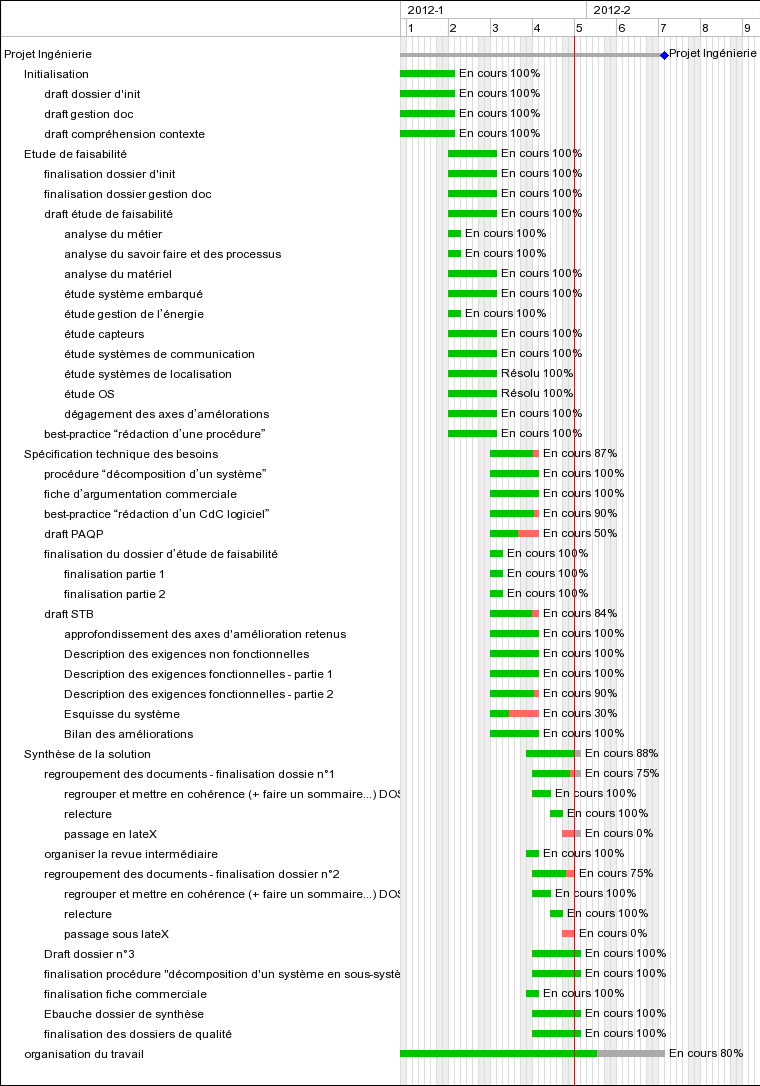
\includegraphics[width=14.579cm,height=20.876cm]{Dossierdinitialisationgestion-img1.png}

\end{document}
